\chapter{Experimentos, resultados e discussão}
\label{sec::experimentos}

Neste capítulo, mostramos os experimentos e resultados do algoritmo de renderização proposto, bem como as funcionalidades adicionadas ao longo do tempo objetivando a interatividade.

Na Seção \ref{sec::glifos_odf_visualizacao_multimodal}, descrevemos os experimentos e resultados do algoritmo de renderização glifos ODF integrados ao ambiente de visualização multimodal. Na Seção \ref{chap::renderizacao_de_perfis_de_difusao}, apresentamos um ambiente de testes e abordamos a evolução do algoritmo de glifos ODFs feitas nesse trabalho, objetivando a interatividade que culminaram no algoritmo de renderização apresentado no Capítulo \ref{chap::renderizacao_interativa_de_perfis_de_difusao}.

Todos os experimentos e medições foram feitas em um computador Macbook Pro Retina 13', com processador Intel Core i5 Dual-Core 2.7GHz, processador gráfico integrado Intel Iris Graphics 6100 1536 MB e memória RAM de 8 GB 1867 MHz DDR3.

\section{Glifos ODF integrados ao ambiente de visualização multimodal}
\label{sec::glifos_odf_visualizacao_multimodal}

Propomos um experimento para avaliar aspectos visuais do nosso algoritmo de esquema de renderização em comparação à superquádricas e medições de performance para atestarmos a interatividade do algoritmo de renderização.

As imagens geradas no experimento foram coletadas a partir o WU-Minn HCP Retest Data pelo \textit{Connectome Project Consortium} \cite{essen2012}.

Os dados de difusão foram adquiridos em um \textit{scanner} Siemens 3T Skyra. A aquisição é \textit{multi-shell} com 90 gradientes de ponderação de difusão para cada \textit{shell} $b = 1000, 2000$ e $3000 s/mm^2$, e estas direções são uniformemente distribuídas nos três \textit{shells}, e adicionalmente foram escaneados 6 aquisições $b0$ para cada \textit{shell}, totalizando 288 volumes. Os dados foram pré-processados com a \textit{pipeline} de pré-processamento para dados de difusão do Human Connectomme Project (HCP) \cite{glasser2013}. A aquisição pré-processada é representada por um volume $145\times 174\times  145$ com espaço entre amostras de $1.25\times 1.25 \times 1.25$mm.

A aquisição anatômica ponderada em T1 foi também pré-processada utilizando a pipeline de pré-processamento do HCP \cite{glasser2013}. Como o seu respectivo DWI, é representada por um volume $145\times 174\times  145$ com espaço entre amostras de $1.25\times 1.25\times 1.25$mm.

As dODFs foram obtidas através do GQI \cite{yeh2010} (Capítulo \ref{chapter::metodos_hardi}) e min-max normalizadas. O fator $\sigma \sqrt{6D}$ que utilizamos é de 0,0239. As amostras foram computadas com base no hemisfério da $8^{a}$ ordem de tesselação do icosaedro e armazenadas na CPU, gerando um total de 321 amostras por \textit{voxel}.

\subsection{Aspectos Visuais}
\label{ssec::aspectos_visuais}

\subsection{Transição de Resolução}

Com o objetivo de evidenciar a diferença na resolução e quantidade de triângulos nas transições das malhas esféricas base, fizemos um experimento em que interagimos com o ambiente de visualização multimodal em que modificamos ajustamos o fator de escala na visualização tal que o $max_p$ mensurado esteja no limite da troca da malha esférica utilizada no glifo. Fig.  \ref{fig::multimodal_teste_zoom} ilustra experimento.

Fig. \ref{fig::multimodal_162_hollow} e \ref{fig::multimodal_642_hollow} correspondem aos mesmos glifos em Fig. \ref{fig::multimodal_162_filled} e \ref{fig::multimodal_642_filled}, respectivamente e estão apresentados para evidenciar a mudança na quantidade de triângulos em cada um deles. As imagens foram gerada a partir de uma janela $500 \times 500$ com uma diferença sutil no fator de escala entre ambas. Nas Fig. \ref{fig::multimodal_162_hollow} e \ref{fig::multimodal_162_filled}, o valor de $max_p$ é de 1394 \textit{pixels}, e em \ref{fig::multimodal_642_hollow} e \ref{fig::multimodal_642_filled}, é de 1409. De acordo com Eq. \ref{eq::icosa_order}, o limiar de mudança entre as geometrias é $max_p = 1406.25$.  O glifo mostra uma visão axial do corpo caloso, cujo comportamento de difusão ocorre predominantemente na direção esquerda-direita. Fig. \ref{fig::multimodal_teste_loc} mostra a localização da região mostrada em Fig. \ref{fig::multimodal_teste_zoom}.


\begin{figure}[ht]
    \centering
    %\rule{6cm}{3cm}
    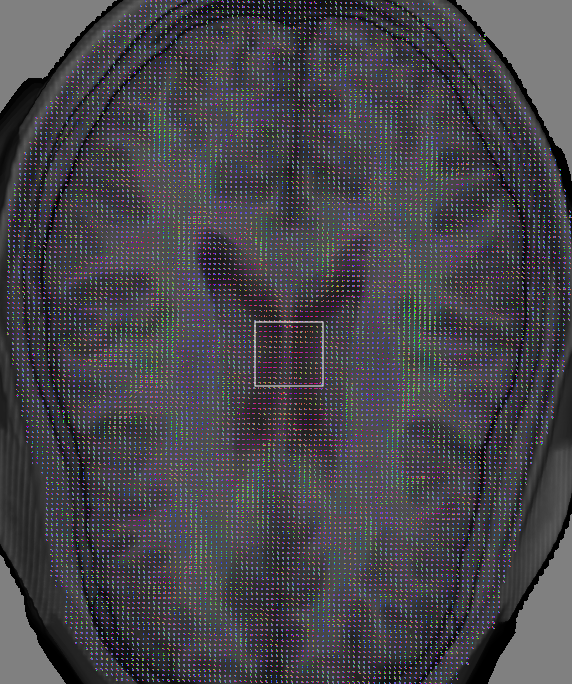
\includegraphics[width=.56\linewidth, angle=0]{figs/Esquema_Glifo/Teste_transicao/base_teste_zoom.png}
    \caption{MRI T1 anatômico co-registrado com DWI. A região dentro do contorno quadrado branco corresponde a região analisada na Fig. \ref{fig::multimodal_teste_zoom}.}
    \label{fig::multimodal_teste_loc}
\end{figure}


\begin{figure}[ht]
\centering
\captionsetup[subfloat]{farskip=0pt,nearskip=0pt}
    \subfloat[$4^a$ ordem de tesselação - apenas contornos dos triângulos]{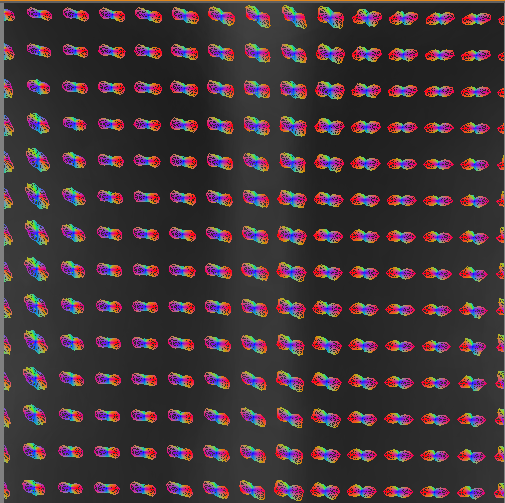
\includegraphics[width=.49\linewidth, angle=0]{figs/Esquema_Glifo/Teste_transicao/162_Hollow.png}
    \label{fig::multimodal_162_hollow}
    }
    \subfloat[$4^a$ ordem de tesselação - triângulos preenchidos] {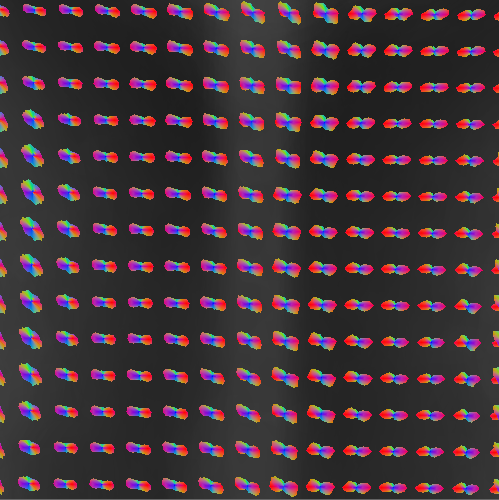
\includegraphics[width=.485\linewidth, angle=0]{figs/Esquema_Glifo/Teste_transicao/162_filled.png}
    \label{fig::multimodal_162_filled}
    }
    \hspace{1pt}
    \subfloat[$8^a$ ordem de tesselação - apenas contornos dos triângulos]{\includegraphics[width=.495\linewidth, angle=0]{figs/Esquema_Glifo/Teste_transicao/642_Hollow.png}
    \label{fig::multimodal_642_hollow}
    }
    \subfloat[$8^a$ ordem de tesselação - triângulos preenchidos] {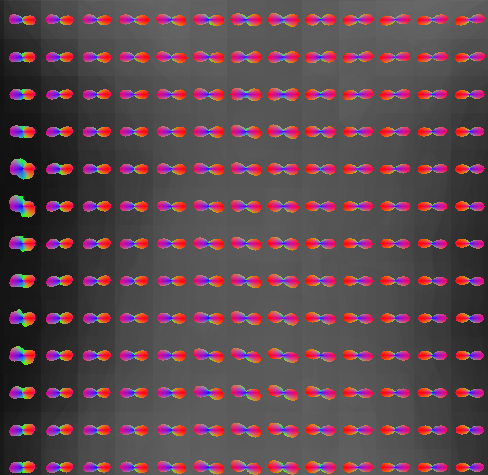
\includegraphics[width=.487\linewidth, angle=0]{figs/Esquema_Glifo/Teste_transicao/642_filled.png}
    \label{fig::multimodal_642_filled}
    }
    \caption{Ilustração da troca de resolução efetuada automaticamente a partir de $max_p$. A troca de resolução ocorre entre as geometrias base derivadas da $4^a$ (\ref{fig::multimodal_162_hollow} e \ref{fig::multimodal_162_filled}) e $8^a$ (\ref{fig::multimodal_642_hollow} e \ref{fig::multimodal_642_filled}) ordem de tesselação. A região ilustrada é do corpo caloso, que está em destaque na Fig. \ref{fig::multimodal_teste_loc}.
    }
    \label{fig::multimodal_teste_zoom}
\end{figure}

Podemos observar a suavidade em que a mudança de resolução ocorre. Observamos que os glifos com os triângulos preenchidos neste nível de resolução não apresentam efeitos característicos de malhas de baixa resolução e que a transição na resolução ocorre de forma sutil.

Adicionalmente, caso o usuário queira analisar os glifos mais de perto ou aumente o tamanho da janela, fazendo-a cobrir mais \textit{pixels}, o glifo é gerado a partir de uma malha suave o suficiente no qual ele tenha total liberdade para visualizar o comportamento das ODFs. Caso o usuário queira ter uma visão mais geral do volume com os glifos e diminua o fator de escala, diminuímos a resolução de cada glifo renderizado para aliviar o processamento computacional associado a cada um deles.


\subsubsection{Cruzamentos de Fibras}

Fig. \ref{fig::multimodal} ilustra uma fatia coronal na região do \textit{centrum semiovale} com um triplo cruzamento de fibras correspondentes do corpo caloso, \textit{corona radiata} e o fascículo longitudinal superior. A região apresenta cruzamentos de fibra conhecidos e é utilizada para análises qualitativas. Fig. \ref{fig::multimodal_highres} mostra que pode-se inferir sobre cada cruzamento de fibra nas regiões mais alongadas da superfície do glifo. Observe também que a resolução do glifo é diferente na Fig. \ref{fig::multimodal_lowres} em comparação a \ref{fig::multimodal_highres} e sua seleção é feita de forma automática. No fundo, há a renderização da ressonância anatômica ponderada em T1 co-registrada.

\begin{figure}[ht]
\centering
\captionsetup[subfloat]{farskip=0pt,nearskip=0pt}
    \subfloat[Fatia coronal de um MRI T1 co-registrado com DWI. A malha esférica base corresponde a $2^a$ ordem de tesselação do icosaedro.]{\makebox[1.2\width]{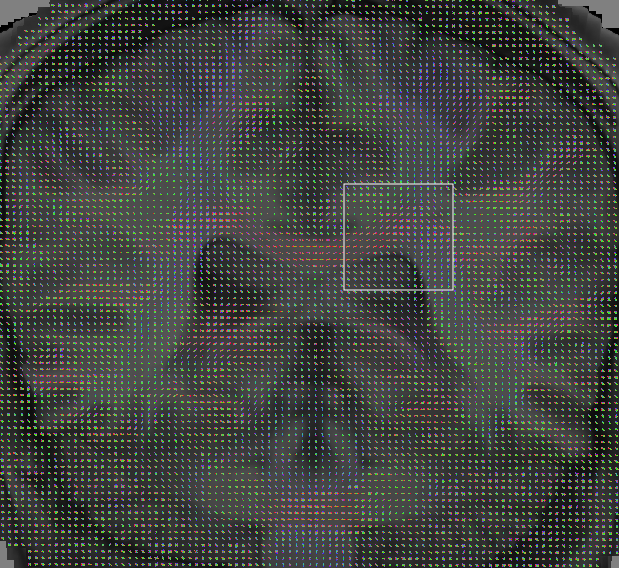
\includegraphics[width=.60\linewidth, angle=0]{figs/Esquema_Glifo/LowResImgHighlighted.png}}
    \label{fig::multimodal_lowres}
    }
    \hspace{1pt}
    
    \subfloat[Cruzamento entre fibras de corpo caloso (esquerda-direita), \textit{corona radiata} (descendente-ascendente) e fascículo longitudinal superior (anteroposterior - normal ao plano da página). A malha esférica base é a $8^a$ ordem de tesselação do icosaedro.] {\makebox[2.0\width]{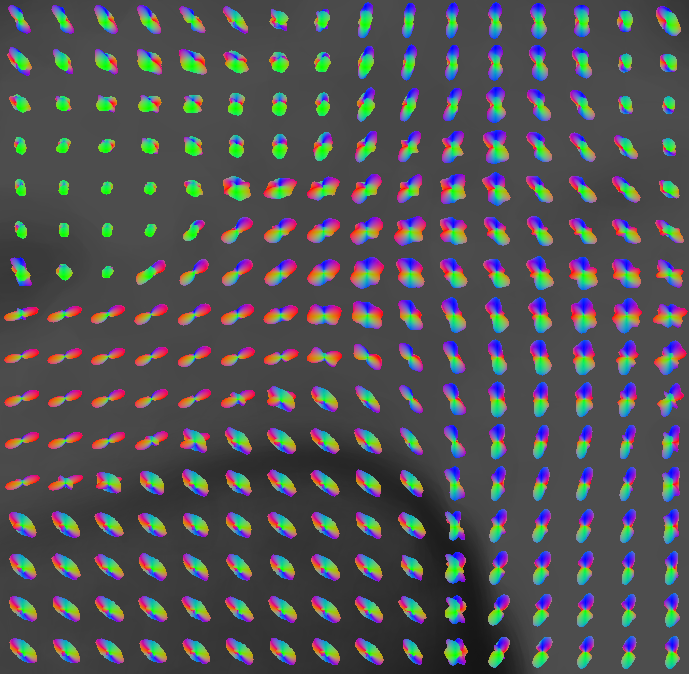
\includegraphics[width=.45\linewidth, angle=0]{figs/Esquema_Glifo/HighResImg.png}
    \label{fig::multimodal_highres}}
    }
    \caption{Glifos ODF integrados ao ambiente de visualização multimodal para MRI. A imagem se refere a um MRI T1 cor-registrado a o seu respectivo DWI. \ref{fig::multimodal_highres} corresponde a região dentro do contorno de cor branca em \ref{fig::multimodal_lowres}.}
    \label{fig::multimodal}
\end{figure}



\citeonline{voltoline2021} evidenciaram que a sua respectiva renderização multimodal para superquádricas do DTI pode ajudar no processo de escolhas referentes a sementes em tractografia, em comparação à mapas de anisotropia codificados por cor. Fig. \ref{fig::multimodal_superquadric} ilustra a mesma região de Fig. \ref{fig::multimodal_highres} com superquádricas. Note que os glifos apresentam o mesmo problema presente no próprio DTI: em cruzamentos de fibra, a distribuição de fibras subjacente não é inferível. Pode-se perceber isto na região de cruzamento de fibras enquanto nos glifos ODF, é possível inferir sobre a natureza do cruzamento de fibras, nas superquádricas, o glifo apresenta uma forma retangular suave e não gera a possibilidade de inferir sobre as fibras que compõem o cruzamento.


\begin{figure}[ht]
    \centering
    %\rule{6cm}{3cm}
    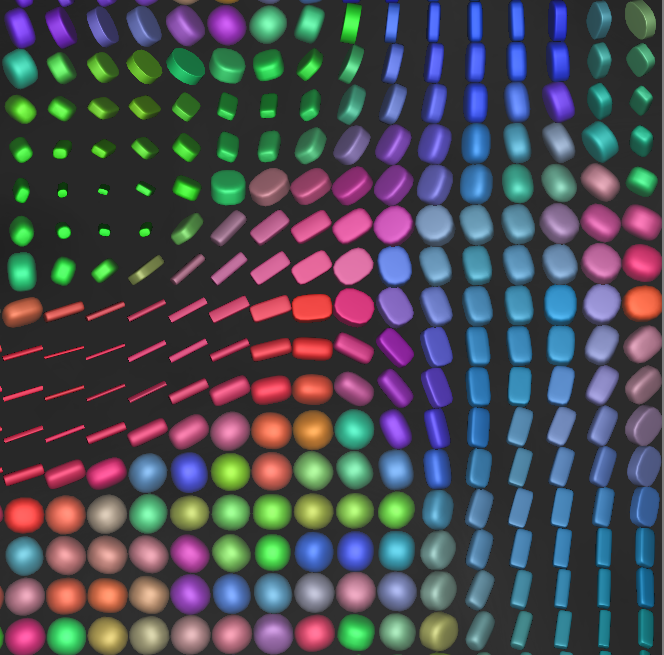
\includegraphics[width=.35\linewidth, angle=0]{figs/Esquema_Glifo/HighResImgSuperquadric.png}
    \caption{ Renderização multimodal para superquádricos do DTI. A imagem corresponde à mesma região em Fig. \ref{fig::multimodal_highres}.}
    \label{fig::multimodal_superquadric}
\end{figure}

\subsection{Performance}
\label{ssec::performance}

Mensuramos o tempo de performance da renderização multimodal de glifos para ODF. O número de glifos é modificado pela mudança do fator de \textit{zoom}. Evidentemente que, maior o fator de \textit{zoom}, menor a quantidade de glifos, maior é a ocupação dos \textit{voxels} na tela, o que aumenta a resolução do glifos. A resolução da janela de saída é de $850\times 850$ e o número de glifos visíveis varia de 12 e 13205. A resolução dos glifos varia com a utilização da $2^a$ ordem de tesselação do icosaedro (menor nível de detalhe, Fig. \ref{fig::multimodal_lowres}) até a $8^a$ (maior nível de detalhe, Fig. \ref{fig::multimodal_highres}). O FPS do esquema de renderização em função da quantidade de glifos renderizados e parâmetros relacionados de fator de escala e ordem de tesselação utilizados estão listados na Tabela \ref{tab::glyph_info_experiment}, onde atestamos que o esquema renderiza em taxas interativas \cite{nielsen1994}.



\begin{table}[ht]
\centering
\begin{tabular}{|cccc|}
\hline
\textbf{FPS} & \textbf{Fator de escala} & \textbf{\# glifos} & \textbf{\begin{tabular}[c]{@{}c@{}}Ordem de \\ tesselação\end{tabular}} \\ \hline
33.85 & 92.27 & 12     & 8 \\
33.69 & 61.51 & 20     & 8 \\
34.75 & 41.01 & 42     & 8 \\
34.66 & 27.34 & 90     & 8 \\
36.29 & 18.23 & 182    & 8 \\
35.97 & 12.15 & 380    & 8 \\
32.98 & 8.10  & 870    & 4 \\
35.83 & 5.40  & 1892   & 4 \\
31.92 & 3.60  & 4160   & 4 \\
22.94 & 2.40  & 9032   & 4 \\
17.15 & 1.52  & 13205  & 2  \\
\hline
\end{tabular}
\caption{Esquema de renderização multimodal com glifos de ODF renderizados em uma imagem $850\times 850$. O número de vértices e triângulos utilizados são computados de acordo com as Eq. \ref{eq::icosphere_vertices} e \ref{eq::icosphere_triangulos}. A Fig. \ref{fig::qualidade_visual_longe_lowres} do apêndice se refere a imagem gerada pelos parâmetros da última linha da tabela}
\label{tab::glyph_info_experiment}
\end{table}

\subsection{Renderização por Fatias}
\label{ssec::renderizacao_por_fatias}

Podemos comparar nossa abordagem com a de \citeonline{shattuck2008}, uma vez que ambas são baseadas em polígonos, onde amostras de ODF deformam uma malha esférica. Em sua abordagem, \citeonline{shattuck2008} armazena ODFs como coeficientes de funções base na CPU e os glifos são computados e visualizados em fatias, que são visualizadas de forma ortogonal. O cômputo da forma dos glifos é feito na CPU, onde o valor de ODF é computada para as normais dos vértices da malha esférica utilizada, deslocando cada um dos vértices, e o tráfego CPU-GPU consiste no envio de dados de vértices de forma que sua estrutura de dados define a superfície do glifo.

Em nossa abordagem, setamos a malha esférica de amostragem a priori e armazenamos amostras de dados de ODF e mostramos estratégias para escolher a malha esférica adequada e estratégias para lidar com o gargalo de tráfego de dados CPU-GPU. Para atingir este objetivo, mostramos formas de organizar os dados de ODF e da malha esférica de amostragem para utilizar renderização por instâncias, técnica que não estava disponível quando \citeonline{shattuck2008} publicaram seu trabalho\footnote{Em OpenGL, renderização por instâncias foi disponibilizada a partir da versão 3.2, lançada em 2009}. Adicionalmente, no processo de renderização, apenas enviamos um conjunto de escalares de ODF para deslocar a malha esférica escolhida e deslocamos os pontos da malha nas \textit{threads} da GPU. Assim, o tráfego de dados por glifo é de $N/2 + (4-N/2 \mod{4})$ \textit{floats} para uma geometria base com $N$ vértices. A possibilidade de diminuir o tráfego de dados por glifo para esta quantidade tem sido crucial para renderizar este glifos com malhas suaves em taxas interativas. Adicionalmente, os glifos são renderizados com apenas um comando de desenho e sua quantidade máxima é limitada pelo máximo número de elementos permitidos em uma das dimensões da textura 2D.

Uma vez que nossa abordagem é vinculada à renderização de um volume via \textit{ray-casting}, apenas os \textit{voxels} visíveis são requisitados a serem desenhados, e não há a restrição a uma fatia inteira. Além disso, no ambiente interativo de visualização, onde o usuário tem a possibilidade de mudar a escala e mover o volume, a detecção de \textit{voxels} visíveis certifica que os \textit{voxels} que estão fora da cena não são demandados na renderização, consequentemente, seus dados não são enviados à GPU e nem são processados no \textit{vertex shader} para serem descartados na rasterização.

Nosso esquema é também aplicável em renderização de glifos baseada em fatia. Observe que, o conjunto $D$ pode se referir a um conjunto de índices referentes a \textit{voxels} que definem uma fatia. Adicionalmente, os atributos de translação podem posicionar os glifos em um \textit{grid} $W \times H$, onde este atributo posiciona cada objeto ao centro de cada célula, que é escalonado pelo fator que o faz estar contido.

%Objetivando gerar resultados de performance do algoritmo e renderização em uma fatia 2-D, fizemos o seguinte experimento: os eixos x e y são divididos em $H$ intervalos ($W = H$), gerando o total de $H^2$ células quadriculadas, no qual glifos são renderizados em cada uma delas. Cada glifo é escalonado para estar contido em sua respectiva célula e posicionado em seu centro. Fixamos a geometria base, assim como os atributos de translação e, para evidenciar a interatividade do algoritmo sob a circunstância de uma frequente troca de fatias, a cada requisição de desenho, os atributos de translação e a matriz de amostras de ODF são preparados e enviados à GPU, conforme mostrado na Subseção \ref{ssec::atributos}.

%Mensuramos o FPS como uma função da quantidade de glifos renderizados com $H$ variando de 5 até 100. O gráfico de $FPS \times \text{glifos renderizados}$ é ilustrado na Fig. \ref{fig::slice_benchmark} para diferentes geometria base utilizadas em uma janela $1200\times 1200$.

% \begin{figure}[htb]
%     \centering
%     %\rule{6cm}{3cm}
%     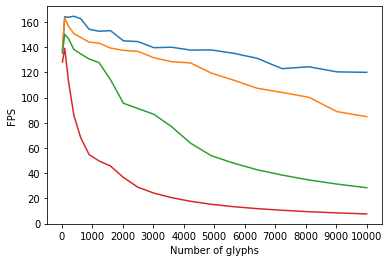
\includegraphics[width=.65\linewidth, angle=0]{figs/Esquema_Glifo/benchmark_half_texopt.png}
%     \caption{FPS $\times$ quantidade de glifos renderizada. As cores azul, laranja, verde e vermelha correspondem a geometria base gerada pela $2^{a}$ $4^{a}$, $8^{a}$ e $16^{a}$ ordem de tesselação do icosaedro. Suas respectivas quantidades de vértices e triângulo são computadas nas Eq. \ref{eq::2ordem_icosphere_vertices} e \ref{eq::2ordem_icosphere_triangulos}, respectivamente.}
%     \label{fig::slice_benchmark}
% \end{figure}

%Os resultados indicam que nosso esquema dá resultados satisfatórios para uso interativo, e mostramos que é possível renderizar milhares de glifos em taxas interativas utilizando a $4^{a}$ ordem de tesselação do icosaedro e centenas com a malha suave gerada pela $16^{a}$ ordem de tesselação.

Na próxima seção, descrevemos uma infra-estrutura fora do ambiente de renderização multimodal para renderização de glifos ODF no qual a utilizamos para fazer testes e validações da melhora do algoritmo. Nela, apresentamos o primeiro protótipo do algoritmo, no qual tem semelhanças com o trabalho de \citeonline{shattuck2008} e as funcionalidades adicionadas ao longo do tempo. Para mensurar ganhos obtidos para cada funcionalidade adicionada, mensuramos o FPS do algoritmo para diferentes quantidade de glifos renderizadas para diferentes resoluções e comparamos com à abordagem anterior.

%Objetivando gerar resultados de performance do algoritmo e renderização em uma fatia 2-D, fizemos o seguinte experimento: os eixos x e y são divididos em $H$ intervalos ($W = H$), gerando o total de $H^2$ células quadriculadas, no qual glifos são renderizados em cada uma delas. Cada glifo é escalonado para estar contido em sua respectiva célula e posicionado em seu centro. Fixamos a geometria base, assim como os atributos de translação e, para evidenciar a interatividade do algoritmo sob a circunstância de uma frequente troca de fatias, a cada requisição de desenho, os atributos de translação e a matriz de amostras de ODF são preparados e enviados à GPU, conforme mostrado na Subseção \ref{ssec::atributos}.


%, no qual foi aperfeiçoado por \cite{almsick2011}. Esta abordagem possibilitou incrementos em performance em relação a \citeonline{shattuck2008}.

%\citeonline{raphael_dissertacao} propôs um esquema de renderização interativa do tensor de difusão em glifos superquádricos \cite{Kindlmann2004} utilizando polígonos. Em seu trabalho, os glifos são renderizados a taxas interativas e a sua abordagem consiste na minimização de tráfego de dados entre CPU-GPU, que consiste apenas em parâmetros que customizam e deslocam os glifos, e o uso de renderização por instâncias. Adicionalmente, este esquema está integrado ao VMTK-Neuro. Os resultados obtidos neste trabalho nos influenciou a adaptar o seu esquema para glifos HARDI.



%\subsection{\sout{Abordagem de renderização}}

%\sout{\citeonline{peeters2009} apresentou pela primeira vez um esquema de renderização para esta categoria de glifos, nos quais são aperfeiçoados por \citeonline{almsick2011} e \citeonline{hlawitschka2012}. Estes esquemas utilizam a abordagem \textit{raycasting}.}

%\sout{No VMTK-Neuro, um dos algoritmos de renderização do tensor difusão por glifos superquádricos é feita por instanciações de uma malha esférica, no qual é customizada por parâmetros particulares a cada tensor de difusão referentes a cada \textit{voxel} detectado e posicionado na cena de acordo. Este esquema de renderização desenha os glifos em tempo interativo.}

%\sout{Pela maior simplicidade e boa efetividade da renderização por instanciações de uma malha esférica, o esquema desenvolvido neste trabalho utiliza esta abordagem.}



%Dados relativos ao desempenho \sout{serão mais detalhados na dissertação de mestrado}\textcolor{blue}{estão disponíveis no link ...}.



%\sout{Medições do tempo relativo ao desempenho foram feitas para a quantidade de 197 vértices da malha esférica \sout{em um}\textcolor{blue}{num} volume de resolução 128x128x90. Para uma quantidade na faixa de 5000 glifos renderizados simultaneamente sobre uma fatia completa, obtemos tem um tempo de resposta entre 80 e 110ms. Para uma quantidade pequena de glifos na faixa das dezenas, o tempo de resposta cai para o intervalo entre 60 e 70ms. Esse tempo de resposta está nas proximidades ou é menor do que o tempo de 0,1s, que é o limite máximo para que o usuário tenha a percepção de resposta instantânea da máquina e que suas ações são a causa de que algo aconteça na tela \cite{nielsen1994}.}

%\sout{No cômputo das ODFs do \textit{QBall}, é feito o mapeamento do sinal de DWI para a ODF a partir das direções derivadas da malha esférica. O glifo para visualização é gerado diretamente de acordo a representação gráfica polar esférica em que $R(\textbf{u}) = R(\mathbf{u})$, onde \textbf{u} é a direção de difusão. A malha esférica utilizada para geração dos glifos em \ref{section::QBall_Glifos} está representada na figura \ref{fig::MalhaEsferico}.}

%A priori, todas as ODFs são calculadas e normalizadas para o intervalo $[0,1]$ para cada um dos \textit{voxels} do volume e referenciadas no processo de renderização.

%O formato de armazenamento dos valores ODF associados à malha consiste numa lista de valores escalares associados a cada um dos \textit{voxels}.



%\todo[inline]{Falta uma descrição melhor de como são construídos os glifos a partir de ODFs e o seu mapeamento às entidades gráficas. Isso torna difícil o entendimento da sua implementação. !!Descrito em trabalhos relacionados!}
\section{Funcionalidades adicionadas e ganhos de performance}
\label{chap::renderizacao_de_perfis_de_difusao}

Nesta seção, abordamos a evolução do algoritmo de renderização de glifos ODF feitas neste mestrado objetivando a interatividade. Apresentamos o ambiente de testes, o protótipo inicial e todas as funcionalidades adicionais que implementamos durante o trabalho que culminaram no algoritmo de renderização apresentado no Capítulo \ref{chap::renderizacao_interativa_de_perfis_de_difusao}.

Na Seção \ref{sec::ambiente_teste}, descrevemos o ambiente de teste que implementamos para fazer a validação  de todas as funcionalidades adicionadas no algoritmo de renderização.


Na Seção \ref{sec::primeiro_prototipo}, descrevemos o primeiro protótipo do algoritmo, onde o utilizamos na infraestrutura do ambiente de visualização multimodal para renderização dos glifos. Inicialmente, o protótipo consistiu em uma ferramenta visual para visualização de dados de ODFs em seus respectivos \textit{voxels}.

O primeiro protótipo do algoritmo integrada ao ambiente de visualização multimodal não renderizava de forma interativa, então passamos a explorar ferramentas proporcionadas pela GPU e características da percepção visual humana para que pudéssemos otimizá-lo objetivando a interatividade.

Assim, na Seção \ref{sec::renderizacao_por_instancias} discutimos o uso da instanciação da GPU para renderização dos glifos; na Seção \ref{sec::otimizacao_da_simetria} mostramos como podemos tomar vantagem da simetria das ODFs e melhorar a performance de renderização; na Seção \ref{sec::estrutura_de_dados_para_textura_RGBA} mostramos como podemos minimizar o uso de memória de textura da GPU e seu impacto em performance; e na Seção \ref{sec::adaptatividade_de_resolucao} discutimos como exploramos a percepção visual humana para tornar a resolução dos glifos adaptativa. A ordem de disposição das seções é coerente com a ordem cronológica de integração de cada funcionalidade.

Nas Seções \ref{sec::renderizacao_por_instancias}, \ref{sec::otimizacao_da_simetria} e \ref{sec::estrutura_de_dados_para_textura_RGBA}, fizemos a validação da funcionalidade adicionada no algoritmo pela comparação gráfica em FPS médio de cada procedimento em relação à seção anterior através do ambiente de teste.% para cada resolução de malha utilizada.

Na Seção \ref{sec::adaptatividade_de_resolucao}, introduzimos a adaptabilidade na resolução como uma função da máxima quantidade de \textit{pixels} contidos em um único \textit{voxel}, o que é algo intrínseco à métricas do ambiente de visualização multimodal. A validação da inserção deste tópico está nos resultados mostrados na Tabela \ref{tab::glyph_info_experiment}, no qual comparamos com o algoritmo de renderização de glifos ODF integrado ao ambiente de visualização multimodal onde a resolução dos glifos é fixa e derivada da $8^a$ ordem de tesselação do icosaedro, que está anotada na Tabela \ref{tab::glyph_info_experiment_fixed}.

%As medições foram feitas em um computador Macbook Pro Retina 13', com processador Intel Core i5 Dual-Core 2.7GHz, processador gráfico integrado Intel Iris Graphics 6100 1536 MB e memória RAM de 8 GB 1867 MHz DDR3. 



\subsection{Ambiente de teste e validação}
\label{sec::ambiente_teste}

Para validar funcionalidades adicionadas que resultam em melhor desempenho no algoritmo de renderização, fizemos um ambiente para testes. Em uma janela de resolução $1200 \times 1200$ \textit{pixels}, dividimos os eixos x e y em $H$ intervalos, gerando $H^2$ células quadradas, nos quais os glifos são renderizados em cada uma delas, conforme mostrado em Fig. \ref{fig::ambiente_validacao}.

Cada glifo é deslocado ao centro da sua respectiva célula e escalonado para caber nela, tendo a sua geometria base fixa. A cada requisição de desenho, todos os atributos de translação e os dados que geram os glifos e que consistem no tráfego de dados CPU-GPU são enviados à GPU, o que é demandado no ambiente de visualização multimodal, conforme mostrado no fluxograma da Fig. \ref{fig::vmtk_simplified}.

\begin{figure}[ht]
\centering
\captionsetup[subfloat]{farskip=5pt,nearskip=0pt}
    %!!VER SE ISSO TA CERTO
    \subfloat[H = 5. 25 glifos renderizados] {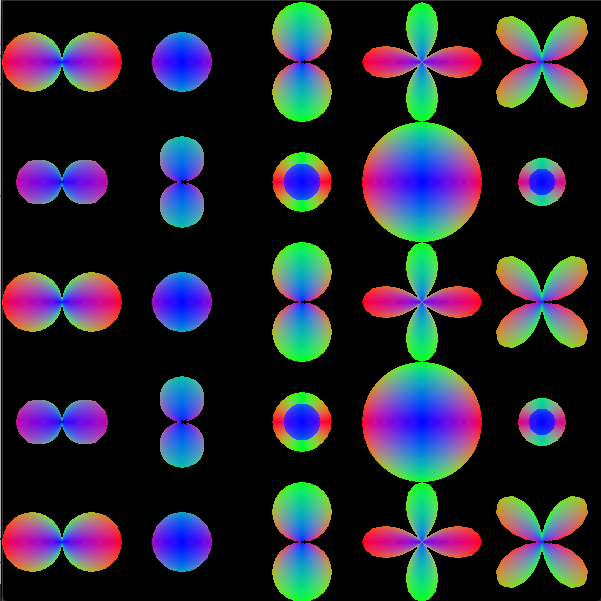
\includegraphics[width=.45\linewidth, angle=0]{figs/Renderizacao_glifos_evolucao/Ilustracao_ambiente/ambiente_5.png}
    \label{fig::ambiente_validacao_5}
    }
    \subfloat[H = 25. 625 glifos renderizados]{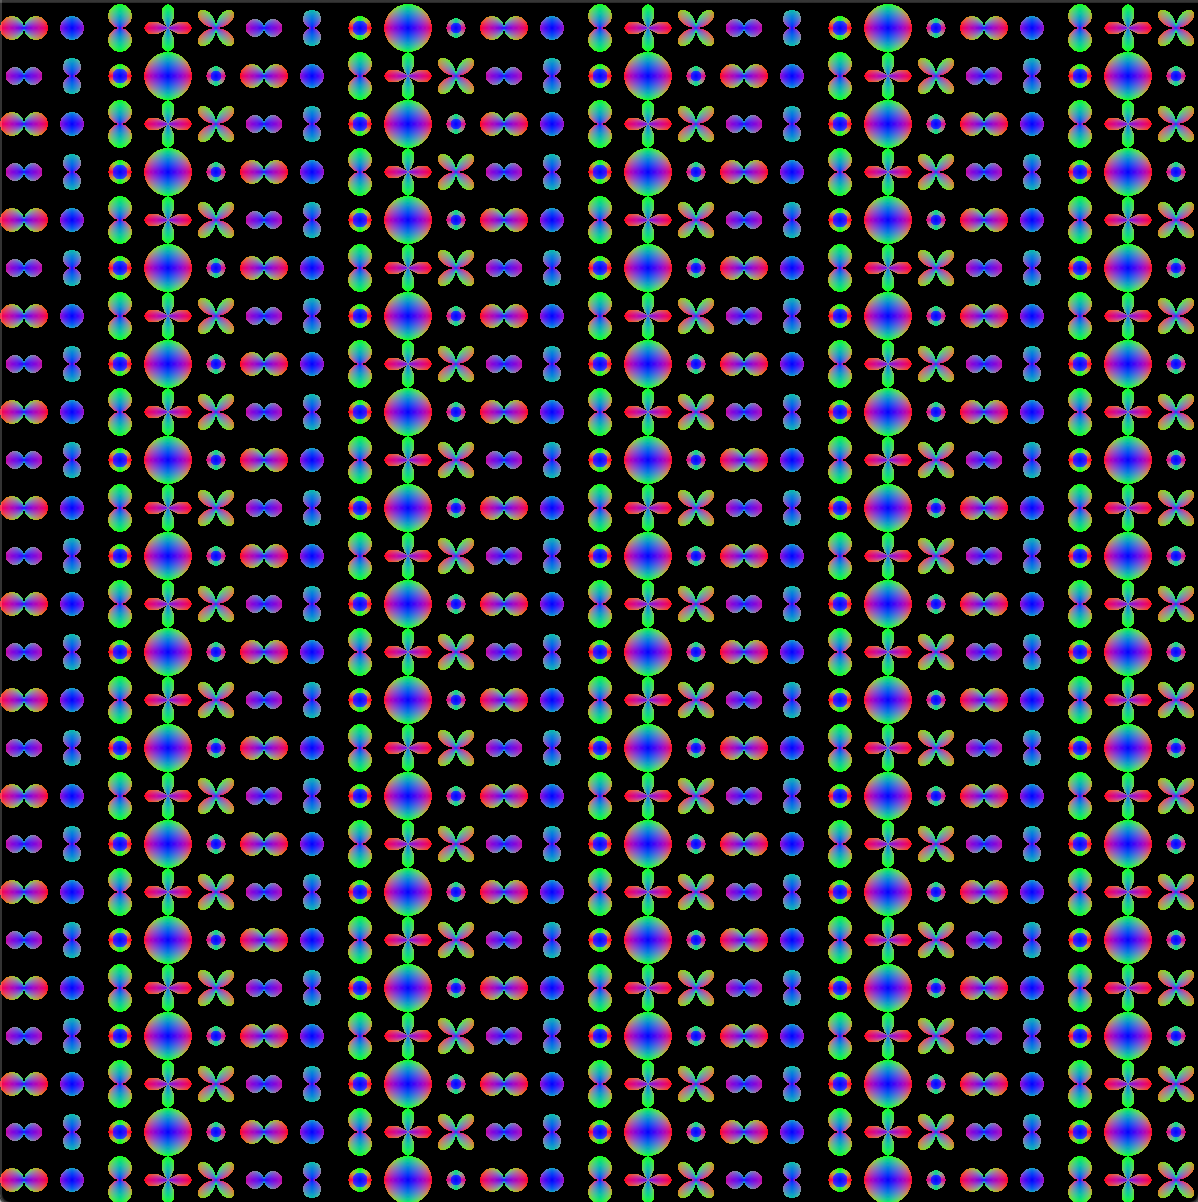
\includegraphics[width=.45\linewidth, angle=0]{figs/Renderizacao_glifos_evolucao/Ilustracao_ambiente/ambiente_25.png}
    \label{fig::ambiente_validacao_25}
    }
    
    \subfloat[H = 50. 2500 glifos renderizados]{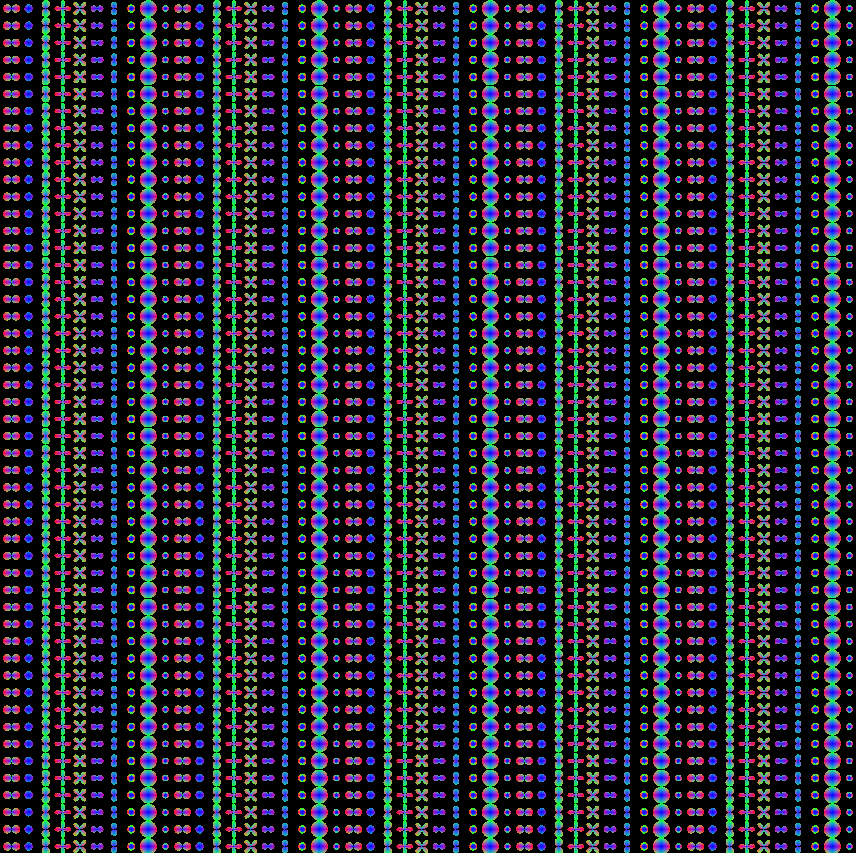
\includegraphics[width=.45\linewidth, angle=0]{figs/Renderizacao_glifos_evolucao/Ilustracao_ambiente/ambiente_50.png}
    \label{fig::ambiente_validacao_50}
    }
    \subfloat[H = 100. 10000 glifos renderizados]{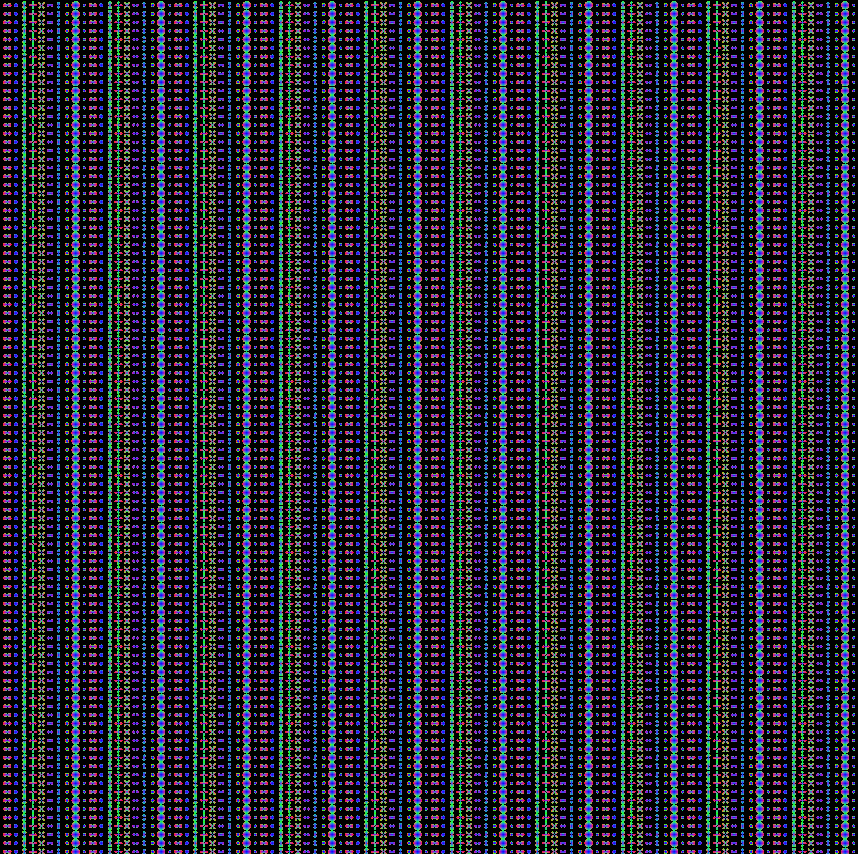
\includegraphics[width=.45\linewidth, angle=0]{figs/Renderizacao_glifos_evolucao/Ilustracao_ambiente/ambiente_100.png}
    \label{fig::ambiente_validacao_100}
    }
     \caption{Ambiente de avaliação do algoritmo de renderização para ODFs. As cores dos glifos referenciam a direção dos eixos de acordo com a Eq. \ref{eq::cor_glifo}.}
    %\hfill
    \label{fig::ambiente_validacao}
\end{figure}

Variamos a quantidade de células $H$ de cinco até cem, anotamos os dados de FPS médio e os mostramos de forma gráfica. Fizemos os experimentos utilizando  as esferas obtidas através da $2^a$, $4^a$, $8^a$ e $16^a$ ordem de tesselação do icosaedro como geometria base.

 No ambiente, as amostras que geram os glifos são computadas a priori a partir de ODFs computadas a partir de funções harmônicas esféricas, cujo o grau das funções varia de zero a três. Utilizamos esta classe de funções porque geram glifos conhecidos\footnote{A página https://chem.libretexts.org/@go/page/283935 oferece a visualização das funções harmônicas esféricas em plotagens polares esféricas.}, o que serviu de suporte para depuração. Esta classe de funções também é comumente utilizada pela comunidade de pesquisa de métodos de alta ordem em DWI \cite{Tournier2004DirectEO, tournier2007, descoteaux2007_QBI}.% e \citeonline{descoteaux2007_QBI} faz uma apresentação delas aplicada a esta área.



Indexamos as células nas quais os glifos são renderizados como $1$, $2$, ..., $M$, cuja sequência é crescente na ordem esquerda para direita, cima e para baixo, e $M = H^2$. Associamos o conjunto de amostras a serem renderizadas na $j$-ésima $(1 \leq j \leq M)$ célula como $\boldsymbol{R}(j) = [
R(j, \mathbf{n}_1), 
R(j, \mathbf{n}_2), 
R(j, \mathbf{n}_3), ..., 
R(j, \mathbf{n}_N)
]^T$, onde $\mathbf{n}_k$ é o vetor unitário com direção e sentido associado à normal do ponto $P_k$ de uma malha esférica $(\Pi, I)$, onde $\Pi = [P_1, P_2, \dots, P_N]$. $I_{3\tau \times 1}$ é o conjunto de índices que triangulam $\Pi$ afim de gerar a malha esférica, onde $\tau$ é a quantidade de triângulos da malha.%\footnote{Escolhemos esta forma de indexar as variáveis envolvidas para que fique similar à forma utilizada no Capítulo \ref{chap::renderizacao_interativa_de_perfis_de_difusao}.}

Utilizamos dez funções harmônicas esféricas, em que, na Fig. \ref{fig::ambiente_validacao_5}, da esquerda para direita e parte superior para inferior, consistem em: $Re(Y_1^{-1})$,
$Re(Y_1^0)$,
$Im(Y_1^{-1})$,
$Re(Y_2^{-2})$,
$Im(Y_2^{-2})$,
$Re(Y_2^{-1})$,
$Im(Y_2^{-1})$,
$Y_2^0$,
$Y_0^0$ e
$Y_3^0$, onde $Y_l^m$ se refere a harmônica esférica de grau $l$ e ordem $m$. Na Seção \ref{sec::harmonicas_esfericas} do Apêndice, escrevemos a formulação analítica das funções utilizadas. Fazemos a associação entre cada $\boldsymbol{R}(j)$, a sua respectiva harmônica esférica de acordo com a Tabela \ref{tab::harmonicas_esfericas}, na qual computamos o seu valor absoluto e fazemos a normalização min-max para o intervalo $[0, 1]$ dos valores amostrados\footnote{No caso da harmônica esférica $(Y_0^0)$, que é constante e mapeada em um glifo esférico, normalizamos a função para ser constante igual a um.}, que são pré-computadas na CPU. Fig. \ref{fig::ambiente_validacao} ilustra os glifos no ambiente de teste para diferentes valores de $M$. O cômputo do valor absoluto torna estas funções simétricas em relação ao eixos coordenados, assim como as funções e sinais de difusão.

\begin{table}[ht]
\centering
\begin{tabular}{cc}
$j \mod 10$ & Harmônica Esférica \\ \hline
1 & $Re(Y_1^{-1})$  \\
2 & $Re(Y_1^0)$     \\
3 & $Im(Y_1^{-1})$  \\
4 & $Re(Y_2^{-2})$  \\
5 & $Im(Y_2^{-2})$  \\
6 & $Re(Y_2^{-1})$  \\
7 & $Im(Y_2^{-1})$  \\
8 & $Y_2^0$         \\
9 & $Y_0^0$         \\
0 & $Y_3^0$        
\end{tabular}
\caption{Associação de índice de célula para função harmônica esférica utilizada. Adicionamos o cômputo dos valores absolutos e fizemos a normalização min-max para cômputo de $\boldsymbol{R}(j)$. Os glifos ODF estão ilustrados em Fig. \ref{fig::ambiente_validacao}.}
\label{tab::harmonicas_esfericas}
\end{table}




\subsection{Primeiro protótipo}
\label{sec::primeiro_prototipo}

No primeiro protótipo, recebendo um conjunto de índices de células cujos glifos ODF são renderizados $D = [
1,
2, ..., 
M
]$, o esquema gera três matrizes $\mathbf{V}$, $I^D$ e $T$ a serem enviados à GPU em função de todas as amostras min-max normalizadas referentes a
$\boldsymbol{R}(1)$,
$\boldsymbol{R}(2)$, ...,
$\boldsymbol{R}(M)$ pré-computadas na CPU. $\mathbf{V}$, se refere ao conjunto de vértices de todos os glifos, $I^D$, se refere ao conjunto de índices que triangulam os vértices dos glifos e $T$ consiste nos dados de translação para as células.

%Para geração dos glifos, uma malha esférica base ($\Pi, I$) é utilizada, Onde $\Pi_{3\times N} = [P_1, P_2, \dots, P_N]$ é o conjunto de vértices da malha, onde $P_k = [P_{xk}, P_{yk}, P_{zk}]^T$, e $I_{3\tau \times 1}$ é o conjunto de índices que triangulam $\Pi$ afim de gerar a malha esférica, onde $\tau$ é a quantidade de triângulos da malha.

%O primeiro vetor, que consistia no conjunto de vértices de todos os glifos renderizados nos seus respectivos sistemas de coordenadas. Para isso, os vértices da malha esférica , $P_k = [P_{xk}, P_{yk}, P_{zk}]^T$ é armazenada e referenciada na CPU.

Na CPU, a matriz $\mathbf{V}_{3\times N\cdot M}$ que contém todos os vértices de todos os glifos é definida. Para isto, cópias dos vértices da malha esférica $\Pi$ são escalonados pelas amostras de ODF dos glifos a serem renderizados, compondo-a, como mostrado na Eq. \ref{eq::vertices_prototipo1}:

\begin{equation}
\label{eq::vertices_prototipo1}
    \mathbf{V} = 
    \begin{bmatrix}
    \Pi\cdot\boldsymbol{R}(1)^D &
    \Pi\cdot\boldsymbol{R}(2)^D &
    \Pi\cdot\boldsymbol{R}(3)^D & \cdots &
    \Pi\cdot\boldsymbol{R}(M)^D
    \end{bmatrix}
    ,
\end{equation}
onde $\boldsymbol{R}(j)_{N\times N}^D$ é a matriz diagonal, onde $\boldsymbol{R}(j)^D[i, i] = \boldsymbol{R}(j, \mathbf{n}_i)$.% em que $\mathbf{n}_i$ é o vetor unitário com direção e sentido da normal de $P_i$.

Também na CPU, o vetor $I_{3 \tau M \times 1}^D$ é definido e consiste na replicação de $I$ para formar as malha esférica esféricas de cada um dos objetos definidos por $\Pi\cdot\boldsymbol{R}(j)^D$. Como todos os glifos são triangulados da mesma forma, $I^D$ consiste em $M$ replicações de $I$ dispostas em sequência, na qual a $j$-ésima replicação consiste na adição de um fator de índice dado por $j\cdot N$. Logo $I^D$ tem a seguinte formulação:
\begin{equation}
\label{eq::index_prototipo1}
    I^D = 
    \begin{bmatrix}
    I \\
    (I +  N\mathbf{1}_{3\tau}  ) \\
    (I + 2N\mathbf{1}_{3\tau} ) \\ \vdots \\ 
    (I + MN\mathbf{1}_{3\tau})
    \end{bmatrix}
    ,
\end{equation}
onde $\mathbf{1_{3\tau}}$ é o vetor coluna com todos os $3\tau$ elementos iguais a um.

Por último e também na CPU, a matriz $T_{3 \times MN}$ consiste no conjunto de atributos de translação, que são aplicados aos vértices dos glifos no \textit{vertex shader}. Para isto, considerando as coordenadas de translação para o centro de cada célula $j$ como $V_j = [V_{jx}, V_{jy}, V_{jz}]^T$, formulamos $T_{3 \times MN}$:

\begin{equation}
\label{eq::translation_prototipo1}
    T_{3 \times MN} =
    \begin{bmatrix}
    V_1 \cdot \mathbf{1}_N^T &
    V_2 \cdot \mathbf{1}_N^T &
    V_3 \cdot \mathbf{1}_N^T & \cdots &
    V_M \cdot \mathbf{1}_N^T
    \end{bmatrix}
,
\end{equation}
onde $\mathbf{1}_N$ é o vetor coluna com todos os N elementos iguais a um.

$\mathbf{V}$, e $T$ são enviados à GPU como atributos e $I^D$ é enviado para referenciar $\mathbf{V}$ e $T$ afim de formar os triângulos. As transformações geométricas feitas na GPU consistem na translação de cada glifo ao centro de sua respectiva célula e escala para cada glifo caber em sua célula, cujo parâmetro é enviado à GPU uma vez como variável uniforme. A renderização é efetuada com apenas um comando de desenho.

%A cor é definida na GPU através da normalização do vértice do glifo no \textit{vertex shader}.%, e há um problema quando ODFs para cômputo direto na GPU de ODFs mapeadas em zero, no qual, neste experimento, quando isso ocorre, mapeamos em branco.

Os resultados em FPS desta abordagem estão mostrado na Fig. \ref{fig::FPS_prototipo_1}. Este protótipo é o mais próximo da abordagem \citeonline{shattuck2008}. A similaridade reside em que os vértices dos glifos são computados na CPU, mas, enquanto na nossa abordagem, as amostras já são pré-computadas, \citeonline{shattuck2008} as computa na CPU em tempo de execução a partir de funções base.% implicando um custo computacional maior para renderização, que é compensado pelo menor uso de memória da CPU, pois os dados de ODF são codificados como coeficientes de funções base.



\begin{figure}[htb]
    \centering
    %\rule{6cm}{3cm}
    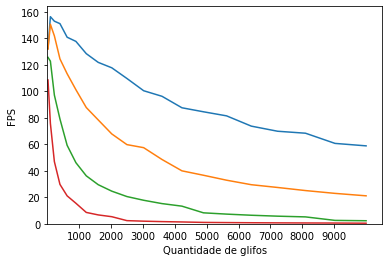
\includegraphics[width=.65\linewidth, angle=0]{figs/Renderizacao_glifos_evolucao/FPS_prototipo1_Geral.png}
    \caption{FPS $\times$ quantidade de glifos renderizada do primeiro protótipo. As cores azul, laranja, verde e vermelha correspondem a geometria base gerada pela $2^{a}$ $4^{a}$, $8^{a}$ e $16^{a}$ ordem de tesselação do icosaedro, respectivamente. Suas quantidades de vértices e triângulo são computadas nas Eq. \ref{eq::icosphere_vertices} e \ref{eq::icosphere_triangulos}, respectivamente.}
    \label{fig::FPS_prototipo_1}
\end{figure}

Esta abordagem gera um tráfego de dados excessivo entre CPU-GPU. Observe que a quantidade de dados por glifo consiste em: $N$ vértices de glifos, $3\tau$ conjunto de índices e $N$ coordenadas de translação. Codificando os vértices e coordenadas de translação em \textit{floats} e o conjunto de índices como inteiro sem sinal, onde cada um destes tipos possui quatro bytes, temos um tráfego CPU-GPU de $24N + 12\tau$ bytes por glifo. Adicionalmente, há uma redundância excessiva na quantidade de dados referentes a translação, e as operações de geração de glifos através do escalonamento dos pontos da esfera podem ser paralelizados, o que torna o uso da GPU para seu cômputo uma potencial vantagem.

Observe que mesmo com o tráfego de dados excessivo, foi possível obter uma taxa de quadros razoável com as subdivisões de $2^a$ e $4^a$ ordem.

%Poderíamos usar $M$ chamadas de desenhos, em que $I$ seria colocado na GPU como um procedimento inicial, e a cada comando de desenho, os dados de vértices dos glifo $d_k$ de ODF são computados e baixados como atributos na GPU; e de translação $V_k$ como uma variável uniforme, levando a um tráfego de $3N + 3$ floats, totalizando $12N + 12$ \textit{bytes}. Mas, o uso de instanciação da GPU, como mostrada na Seção \ref{sec::renderizacao_por_instancias}, provê um tráfego de dados menor, além do uso de apenas um comando de desenho.


\subsection{Instanciação}
\label{sec::renderizacao_por_instancias}

Com o objetivo de diminuir o tráfego de dados e a redundância nos dados de translação, bem como paralelizar o escalonamento dos vértices na malha esférica base afim de obtermos os vértices do glifo, utilizamos renderização por instâncias.

A malha esférica base $(\Pi, I)$ e o parâmetro de escala são enviados à GPU a priori. A malha é instanciada $M$ vezes para os $M$ glifos a renderizar e o parâmetro de escala é enviado como uma variável uniforme. A cada requisição de desenho, parâmetros de ODF min-max normalizada e translação consistem no tráfego de dados CPU-GPU.

O parâmetro de translação deixa de ser um atributo por vértice e se torna um atributo único por instância. Para isso, redefinimos $T$ na CPU, como a seguinte matriz:

\begin{equation}
\label{eq::vertices_prototipo2}
    T_{3\times M} = 
    \begin{bmatrix}
    V_1 & V_2 & V_3 & \cdots & V_M
    \end{bmatrix}
    .
\end{equation}

Definimos a matriz $\boldsymbol{\mathscr{R}}_{N \times M}$, computada na CPU, e que consiste em todas as amostras de ODF que sintetizam os glifos a serem renderizados nas células:%, ilustrada em Eq. \ref{eq::odf_prototipo2}.

\begin{equation}
\label{eq::odf_prototipo2}
\boldsymbol{\mathscr{R}} = 
\begingroup % keep the change local
\setlength\arraycolsep{2pt}
\begin{bmatrix} 
    R(1, \mathbf{n}_1) &
    R(2, \mathbf{n}_1) & \cdots & 
    R(M, \mathbf{n}_1)  \\
    
    R(1, \mathbf{n}_2) &
    R(2, \mathbf{n}_2) & \cdots & 
    R(M, \mathbf{n}_2) \\ \vdots & \vdots & \vdots & \vdots  \\
    
    R(1, \mathbf{n}_N) & 
    R(2, \mathbf{n}_N) & \cdots & 
    R(M, \mathbf{n}_N)
\end{bmatrix}
\endgroup
\end{equation}

Enviamos $\boldsymbol{\mathscr{R}}$ como uma textura 2D, de formato $RED$ e com dimensões $N\times M$. Observe que o acesso na GPU dos elementos pode ser feito a partir dos pares índice de instância e índice de vértice. Na $j$-ésima instância, onde o glifo da $j$-ésima célula é processado, o \textit{lookup} na GPU é feito através da função \textit{texelFetch} das coordenadas não normalizadas $(j, Vertex\_ID)$. O acesso da ODF min-max normalizada no processamento do vértice em sua respectiva instância é feito pela leitura do valor da componente $R$ do $RGBA$ do \textit{texel}.

Após o envio de $\boldsymbol{\mathscr{R}}$ e $T$ à GPU, em adição à Seção \ref{sec::primeiro_prototipo}, o \textit{lookup} de ODFs e o escalonamento dos vértices da malha esférica base efetuada para geração do glifo é feita no \textit{vertex shader} e somente um comando de desenho é efetuado.

Fig. \ref{fig::FPS_prototipo_2} traz os resultados gráficos em FPS de forma comparativa da renderização por instâncias com o primeiro protótipo.

\begin{figure}[htb]
\centering
\captionsetup[subfloat]{farskip=5pt , nearskip=0pt}
    %!!VER SE ISSO TA CERTO
    \subfloat[Tesselação de $2^a$ ordem] {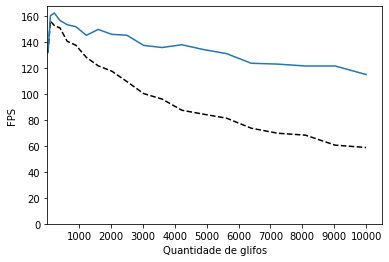
\includegraphics[width=.45\linewidth, angle=0] {figs/Renderizacao_glifos_evolucao/Prototipo2/prototipo_2_42.png}
    \label{fig::FPS_prototipo_2_42}
    }
    \subfloat[Tesselação de $4^a$ ordem] {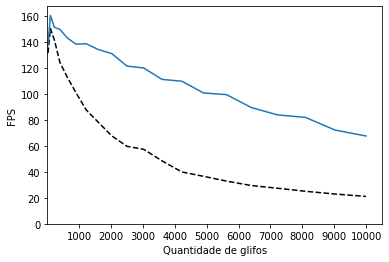
\includegraphics[width=.45\linewidth, angle=0]{figs/Renderizacao_glifos_evolucao/Prototipo2/prototipo_2_162.png}
    \label{fig::FPS_prototipo_2_162}
    }
    
    \subfloat[Tesselação de $8^a$ ordem] {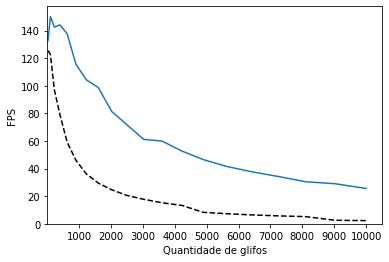
\includegraphics[width=.45\linewidth, angle=0]{figs/Renderizacao_glifos_evolucao/Prototipo2/prototipo_2_642.png}
    \label{fig::FPS_prototipo_2_642}
    }
    \subfloat[Tesselação de $16^a$ ordem] {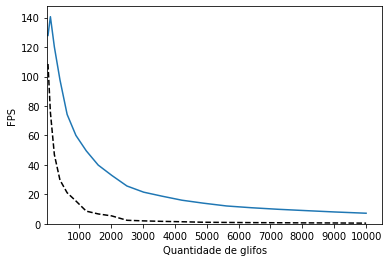
\includegraphics[width=.45\linewidth, angle=0]{figs/Renderizacao_glifos_evolucao/Prototipo2/prototipo_2_2562.png}
    \label{fig::FPS_prototipo_2_2562}
    }
     \caption{FPS $\times$ Quantidade de glifos para diferentes tesselações do icosaedro. A linha preta ilustra o FPS do primeiro protótipo, enquanto a linha azul mostra o FPS da utilização da instanciação da GPU.}
    %\hfill
    \label{fig::FPS_prototipo_2}
\end{figure}


Note que o tráfego de dados CPU-GPU cai drasticamente. Para cada glifo, $N$ valores escalares de ODF são enviados a GPU, adicionalmente, conseguimos sintetizar as coordenadas de translação em um atributo único por glifo, e o conjunto de índices é apenas enviado uma vez, o que elimina o tráfego de dados relacionado a esta variável. Assim, o tráfego de dados por glifo cai para $N + 3$ \textit{floats}, totalizando $4N + 12$ \textit{bytes}. Adicionalmente, a malha esférica base é escalonada para gerar o glifo de forma paralela na GPU.

Note também que, para $8^a$ e $16^a$ ordem de tesselação, o FPS mais que dobra para milhares de glifos renderizados. Observe também que neste ambiente, conseguimos renderizar mais de 3000 glifos em taxas interativas \cite{nielsen1994} a partir da malha suave gerada pela $16^a$ ordem de tesselação do icosaedro. O uso de renderização por instâncias e a diminuição do tráfego de dados de amostras de ODF para apenas amostras escalares enviadas como textura foi o ponto mais crucial neste trabalho rumo a interatividade.

\subsection{Exploração da simetria}
\label{sec::otimizacao_da_simetria}

Nesta seção, exploraremos a simetria das ODFs, i.e. $R(j, \mathbf{n}) = R(j, -\mathbf{n})$, para que possamos diminuir o tráfego de dados de ODF discutidos na Seção \ref{sec::renderizacao_por_instancias}. Para isto, impomos a nossa primeira condição: apenas malhas esféricas com pontos simétricos em relação aos eixos são utilizadas, e os simétricos estão em sequência na memória, ou seja, em $\Pi$, N é par e $P_{2i+2} = -P_{2i+1}$, $(0 \leq i \leq \frac{N-2}{2})$, nos levando a uma estrutura de dados $\Pi = [P_1, -P_1, P_3, -P_3, \dots, P_{N-3}, -P_{N-3}, P_{N-1}, -P_{N-1}]$. Tal como na Seção \ref{sec::renderizacao_por_instancias}, enviamos $(\Pi, I)$ à GPU a priori para ser instanciada $M$ vezes.

Reestruturamos os dados
$\boldsymbol{R}(j)_{N\times 1} = [
R(j, \mathbf{n}_1), 
R(j, \mathbf{n}_2), 
R(j, \mathbf{n}_3), ..., 
R(j, \mathbf{n}_N)
]^T$ para
$\boldsymbol{R}(j)_{\frac{N}{2}\times 1} =[
R(j, \mathbf{n}_1), 
R(j, \mathbf{n}_3), ...
R(j, \mathbf{n}_{N-3}),
R(j, \mathbf{n}_{N-1})
]^T$.

Neste contexto, na formação do glifo ODF na $j$-ésima célula, na i-ésima posição $R(j, \mathbf{n}_{2i-1})$ escalona os pontos $P_{2i-1}$ e $P_{2i}$ da esfera na $j$-ésima instância. Logo, reestruturamos $\boldsymbol{\mathscr{R}}$ para que se torne $\boldsymbol{\mathscr{R}}_{\frac{N}{2}\times M}$, tal que:

\begin{equation}
\label{eq::odf_prototipo3}
\boldsymbol{\mathscr{R}} = 
\begingroup % keep the change local
\setlength\arraycolsep{2pt}
\begin{bmatrix} 
    R(1, \mathbf{n}_1) &
    R(2, \mathbf{n}_1) & \cdots & 
    R(M, \mathbf{n}_1)  \\
    
    R(1, \mathbf{n}_3) &
    R(2, \mathbf{n}_3) & \cdots & 
    R(M, \mathbf{n}_3) \\ \vdots & \vdots & \vdots & \vdots  \\
    
    R(1, \mathbf{n}_{N-1}) & 
    R(2, \mathbf{n}_{N-1}) & \cdots & 
    R(M, \mathbf{n}_{N-1})
\end{bmatrix}
\endgroup
\end{equation}

Assim como na Seção \ref{sec::renderizacao_por_instancias}, enviamos $\boldsymbol{\mathscr{R}}$ à GPU como uma textura 2D, de formato $RED$, com dimensões $\frac{N}{2}\times M$. Observe que o acesso na GPU dos elementos é modificado em função do \textit{Vertex\_ID}. Na $j$-ésima instância, onde o glifo da $j$-ésima célula é processado, o \textit{lookup} na GPU é feito através da função \textit{texelFetch} das coordenadas não normalizadas $\lfloor (j, Vertex\_ID/2)\rfloor$. O acesso da ODF min-max normalizada no processamento do vértice em sua respectiva instância é feito pela leitura do valor da componente $R$ do \textit{texel}\footnote{A função em OpenGL para \textit{lookup} em função dos índices de instância e vértice é dada por texelFetch($\boldsymbol{\mathscr{R}}$,ivec2((gl\_VertexID)/2, gl\_InstanceID), 0).r.}, conforme ilustrado na Fig. \ref{fig::texelfetch_prototipo3}.

\begin{figure}[htb]
%\subfigcapskip = -5pt
    \centering
    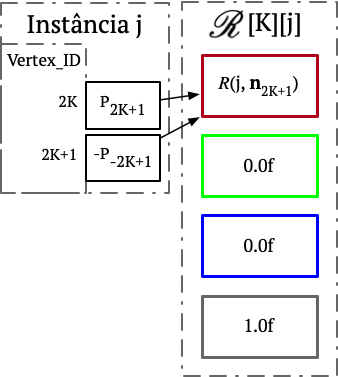
\includegraphics[width=.35\linewidth, angle=0]{figs/Renderizacao_glifos_evolucao/texellookup_RED_4.png}
    \caption{Ilustração do acesso nas componentes RGBA em \textit{texel} na textura \textbf{R} no índice $K$ e $j$. O \textit{texel} é acessado pelas \textit{threads} que processam os vértices de índices 2K e 2K+1 em uma instância $j$. Os blocos de contorno vermelho, azul, verde e cinza ilustram as componentes R,G,B e A do \textit{texel}, respectivamente. Observe que as componentes G, B e A são inicializadas com valores \textit{default}.}
    \label{fig::texelfetch_prototipo3}
   %\hspace{1pt}
\end{figure}


Fig. \ref{fig::FPS_prototipo_3} traz de forma o desempenho em FPS da funcionalidade adicionada nesta seção de forma comparativa à Seção \ref{sec::renderizacao_por_instancias}.

\begin{figure}[H]
\centering
\captionsetup[subfloat]{farskip=5pt,nearskip=0pt}
    %!!VER SE ISSO TA CERTO
    \subfloat[Tesselação de $2^a$ ordem] {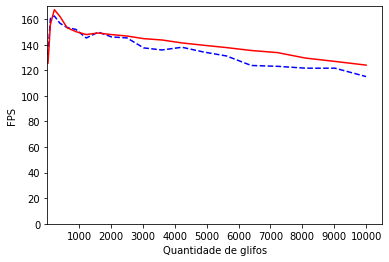
\includegraphics[width=.45\linewidth, angle=0]{figs/Renderizacao_glifos_evolucao/Prototipo3/prototipo_3_42.png}
    \label{fig::FPS_prototipo_3_42}
    }
    \subfloat[Tesselação de $4^a$ ordem] {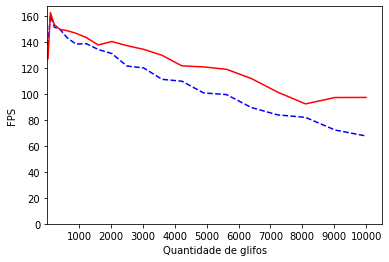
\includegraphics[width=.45\linewidth, angle=0]{figs/Renderizacao_glifos_evolucao/Prototipo3/prototipo_3_162.png}
    \label{fig::FPS_prototipo_3_162}
    }
    
    \subfloat[Tesselação de $8^a$ ordem] {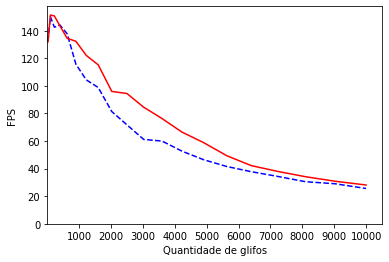
\includegraphics[width=.45\linewidth, angle=0]{figs/Renderizacao_glifos_evolucao/Prototipo3/prototipo_3_642.png}
    \label{fig::FPS_prototipo_3_642}
    }
    \subfloat[Tesselação de $16^a$ ordem] {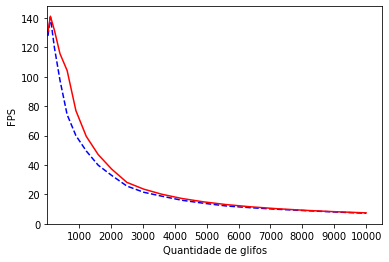
\includegraphics[width=.45\linewidth, angle=0]{figs/Renderizacao_glifos_evolucao/Prototipo3/prototipo_3_2562.png}
    \label{fig::FPS_prototipo_3_2562}
    }
     \caption{FPS $\times$ Quantidade de glifos para diferentes tesselações do icosaedro. A linha pontilhada azul ilustra o FPS do segundo protótipo, enquanto a linha vermelha mostra o FPS quando tomamos vantagem da simetria das ODF.}
    %\hfill
    \label{fig::FPS_prototipo_3}
\end{figure}



Observe que esta otimização faz o tráfego de dados CPU-GPU ser reduzido de $N + 3$ para $N/2 + 3$ \textit{floats}, totalizando $2N + 12$ bytes. Em termos de performance, observe em Fig. \ref{fig::FPS_prototipo_3_642} e \ref{fig::FPS_prototipo_3_2562} que aproximadamente 4900 e 1225 glifos puderam ser renderizados a 60 FPS para $8^a$ e $16^a$ ordem de tesselação, enquanto na abordagem em que não tomamos vantagem da simetria, 3600 e 900 puderam ser gerados.

Por outro lado, observe que os maiores ganhos de performance ocorrem na faixa que compreendem 600 a 1600 glifos para $16^a$ ordem de tesselação e 2400 até 5000 glifos para para $8^a$ ordem, no qual, nesta região, há um ganho em FPS acima de 20\%.

Note que as componentes B, G e A do \textit{texel} são alocadas, setadas para valores padrão e não são utilizadas\footnote{Informações sobre a alocação de memória em uma textura de formato RED e RGBA podem ser encontradas em https://www.khronos.org/registry/OpenGL-Refpages/gl4/html/glTexImage2D.xhtml}. Adicionalmente, as componentes R, G, B e A na memória de textura em cada \textit{texel} estão em sequência na GPU e nesta abordagem, as amostras que sintetizam o glifo estão espaçadas em 3 \textit{floats}. Neste leiaute de memória, no qual os coeficientes de ODF não estão em sequência, alocamos memória em excesso da GPU para valores não utilizados (componentes B, G e A de cada \textit{texel}) e não utilizamos o cache da GPU de forma ótima.



\subsection{Estrutura de dados para textura RGBA}
\label{sec::estrutura_de_dados_para_textura_RGBA}

Para evitar o desperdício de memória e mal uso do cache da GPU, enviamos $\boldsymbol{\mathscr{R}}$ como uma textura de formato RGBA, de tamanho $\lceil \frac{N/2}{4}\rceil \times M$ em que agrupamos os valores escalares da $j$-ésima coluna em sequência de quatro em quatro. Se $N/2$ não é divisível por quatro, é necessária a inserção de linhas com valores \textit{dummy} em $\boldsymbol{\mathscr{R}}$ afim de completar a divisibilidade por quatro, para que cada coluna da matriz possa ser acessada via índice de instância.

Assim, em cada \textit{texel} há quatro amostras de ODF que escalonam 8 pontos da malha esférica. No Capítulo \ref{chap::renderizacao_interativa_de_perfis_de_difusao}, a Fig. \ref{fig::texelfetch} ilustra a forma que o \textit{lookup} é feito, onde neste contexto $j = d_j$. O argumento da função \textit{texelFetch} para a $j$-ésima instância se torna as coordenadas não-normalizadas $(j, \lfloor \frac{Vertex\_ID}{8} \rfloor)$ e o acesso do ponto processado ao seu respectivo valor de ODF min-max normalizado, considerando que as componentes R, G, B e A são mapeados nos índices 0, 1, 2 e 3 nos \textit{texels} é mapeado por $\lfloor Vertex\_ID \mod{8}/2 \rfloor$.

Fig. \ref{fig::FPS_prototipo_4} traz de forma comparativa o FPS gerado por esta nova organização de $\boldsymbol{\mathscr{R}}$ no envio como textura em comparação à Seção \ref{sec::otimizacao_da_simetria}.

\begin{figure}[ht]
\centering
\captionsetup[subfloat]{farskip=5pt,nearskip=0pt}
    %!!VER SE ISSO TA CERTO
    \subfloat[Tesselação de $2^a$ ordem] {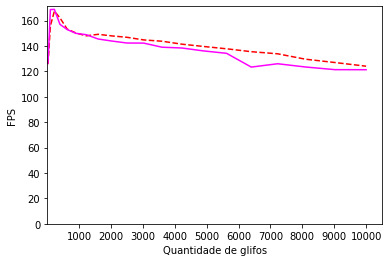
\includegraphics[width=.45\linewidth, angle=0]{figs/Renderizacao_glifos_evolucao/Prototipo4/prototipo_4_42.png}
    \label{fig::FPS_prototipo_4_42}
    }
    \subfloat[Tesselação de $4^a$ ordem] {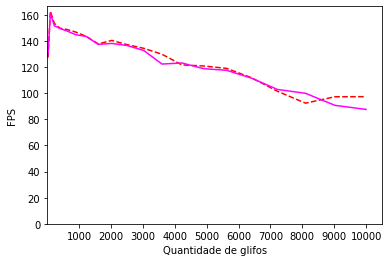
\includegraphics[width=.45\linewidth, angle=0]{figs/Renderizacao_glifos_evolucao/Prototipo4/prototipo_4_162.png}
    \label{fig::FPS_prototipo_4_162}
    }
    
    \subfloat[Tesselação de $8^a$ ordem] {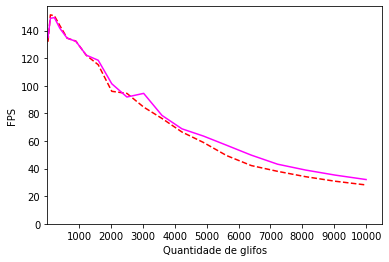
\includegraphics[width=.45\linewidth, angle=0]{figs/Renderizacao_glifos_evolucao/Prototipo4/prototipo_4_642.png}
    \label{fig::FPS_prototipo_4_642}
    }
    \subfloat[Tesselação de $16^a$ ordem] {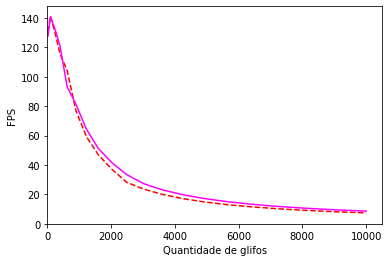
\includegraphics[width=.45\linewidth, angle=0]{figs/Renderizacao_glifos_evolucao/Prototipo4/prototipo_4_2562.png}
    \label{fig::FPS_prototipo_4_2562}
    }
     \caption{FPS $\times$ Quantidade de glifos para diferentes tesselações do icosaedro. A linha pontilhada vermelha ilustra o FPS do terceiro protótipo, enquanto a linha magenta mostra o FPS do uso das componentes RGBA dos \textit{texels} da memória de textura.}
    %\hfill
    \label{fig::FPS_prototipo_4}
\end{figure}


Observe que este procedimento faz o tráfego de dados CPU-GPU ser sutilmente aumentado para $N/2 + 3 + (4 -N/2 \mod{4})$ \textit{floats} por glifo, mas a quantidade de memória alocada para $\boldsymbol{\mathscr{R}}$ na GPU cai para aproximadamente um quarto em comparação à abordagem anterior.

Observe que há um aumento em FPS quando milhares de glifos são renderizados a partir das malhas da $8^a$ e $16^a$ ordem de subdivisão. Na subdivisão de ordem 8, o ganho em FPS é acima de 10\% para mais de 5600 glifos. Na subdivisão de ordem 16, o ganho de FPS é cerca de 10\% para 1600 glifos renderizados e se estabiliza na faixa de 15\% para mais de 5600 glifos renderizados. Por outro lado, a diferença é desprezível quando a quantidade de glifos renderizados é menor que 1000 para estas malhas e totalmente desprezível quando utilizamos as tesselações de ordem dois e quatro.


%Isso ocorre devido a maior alocação de dados de ODF no cache da GPU devido a este procedimento.


\subsection{Adaptatividade de resolução}
\label{sec::adaptatividade_de_resolucao}

Aplicamos todos os conceitos apresentados até a versão do algoritmo de renderização de ODFs, apresentada na Seção \ref{sec::estrutura_de_dados_para_textura_RGBA}, integramos ao ambiente de visualização multimodal e fizemos as medições de performance conforme descrita na Seção \ref{ssec::performance}, onde utilizamos a tesselação de $8^a$ ordem do icosaedro de forma fixa.

No experimento, integramos o algoritmo à estrutura apresentada no Capítulo \ref{chap::renderizacao_interativa_de_perfis_de_difusao}, no qual algoritmo é integrado ao ambiente multimodal e recebe apenas o conjunto de \textit{voxels} detectados como entrada. O cômputo do parâmetro de ocupação do glifo ($max_p$) efetuado na GPU e o algoritmo de escolha da malha esférica base foram desativados para fins de teste. Adicionalmente, usamos o mesmo volume e métodos descrito na Seção \ref{sec::experimentos} do Capítulo \ref{chap::renderizacao_interativa_de_perfis_de_difusao} para gerar os resultados. Os resultados estão apresentados na Tabela \ref{tab::glyph_info_experiment_fixed}.

\begin{table}
\centering
\begin{tabular}{|cccc|}
\hline
\textbf{FPS} & \textbf{Fator de escala} & \textbf{\# glifos} & \textbf{\begin{tabular}[c]{@{}c@{}}Ordem de \\ tesselação\end{tabular}} \\ \hline
34.29 & 86.50 & 12     & 8 \\
35.23 & 58.15 & 20     & 8 \\
35.43 & 38.76 & 42     & 8 \\
35.83 & 25.84 & 90     & 8 \\
32.78 & 17.23 & 182    & 8 \\
35.70 & 11.49 & 380    & 8 \\
32.96 & 7.66  & 870    & 8 \\
28.53 & 5.10  & 1892   & 8 \\
23.17 & 3.40  & 4160   & 8 \\
14.58 & 2.27  & 9166   & 8 \\
 7.96 & 1.51  & 13205  & 8 \\
\hline
\end{tabular}
\caption{Esquema de renderização multimodal com glifos ODF renderizados em uma imagem $850\times 850$ com a malha esférica base fixa. A última linha da tabela descreve a geração da imagem na Fig. \ref{fig::qualidade_visual_longe_highres} no apêndice.}
\label{tab::glyph_info_experiment_fixed}
\end{table}

Observe que não conseguimos renderizar os glifos em taxas interativas quando há muitos deles sendo renderizados e para resolver este problema, resolvemos tornar a malha esférica base dos glifos adaptativa. Assim, dividimos este problema em duas partes: (1) como podemos alternar geometrias base para sub-malhas de malha esférica base em tempo de execução; e (2) como podemos diminuir o tráfego de dados para que apenas os dados referentes às sub-malhas sejam enviados à GPU.

Com este objetivo, propomos a segunda condição que restringe o uso da malha esférica base $(\Pi, I)$: $(\Pi, I)$ se torna $(\Pi, I_k)$ e tem $k$ sub-malhas, onde cada sub-malha é denotada por $(\Pi_i, I_i)$,  $(0 \leq i \leq k)$. Adicionalmente, o número de pontos das sub-malhas é crescente de acordo com os sub-índices, i.e. se $(0 \leq i < j < k)$, implica $|\Pi_j| > |\Pi_i|$. Os primeiros $|\Pi_i|$ elementos na estrutura de dados de $\Pi$ corresponde aos elementos de $\Pi_i$. Note que esta condição também implica que, para $i$, $j$ tais $0 \leq i < j < k$, $\Pi_i$ é subconjunto de $\Pi_j$.

Aplicadas estas condições, resolvemos a alternância de malhas esféricas, fazendo com que, no processo de inicialização do algoritmo de renderização, os conjunto de vértices $\Pi$ e os conjunto de índices $I_0$, $I_1$, ..., $I_{k-1}$, $I_k$ sejam carregados na GPU.

Resolvemos o problema de tráfego de dados no envio das amostras, no qual as amostras que deformam a sub-malha esférica de mais baixa resolução são colocadas na parte inicial de $\boldsymbol{R}(\mathbf{r})$, as amostras que deformam a sub-malha esférica de segunda mais baixa resolução, envolve as amostras da primeira e as suas próprias amostras em $\boldsymbol{R(\mathbf{r})}$, e assim por diante.

Sugerimos tesselações do icosaedro de ordem potência de dois para este fim, no qual propomos que os vértices do icosaedro consistam nos primeiros 12 vértices da estrutura de dados, a subdivisão de $2^a$ ordem consista nos 42 primeiros vértices, a subdivisão de $4^a$ ordem consista nos primeiros 162 vértices na estrutura de dados, e assim sucessivamente\footnote{A Eq. \ref{eq::icosphere_vertices} formula a quantidade de vértices em função da ordem de tesselação.}. Adicionalmente, as antípodas estão dispostas de forma consecutiva na memória no conjunto de vértices $\Pi$, assim como nas Seções \ref{sec::otimizacao_da_simetria} e \ref{sec::estrutura_de_dados_para_textura_RGBA}.

A forma que escolhemos para fazer a escolha entre uma destas é baseado na relação heurística de \citeonline{voltoline2021}, que estabelece uma quantidade mínima de triângulos para manutenção de uma boa qualidade visual dos glifos, dado a sua ocupação em \textit{pixels}, que está formulada na Seção %\ref{sssec::formulação_da_geometria_e_estruturação_de_dados}, 
\ref{malha_esferica}. A quantidade de amostras enviadas à GPU para customizar o glifo das sub-malhas se torna adaptativa, na Seção \ref{sec::renderizacao_de_glifos_ODF}, estruturamos os dados afim de gerar essa adaptabilidade e na Seção \ref{ssec::preparacao_de_dados}, aproveitamos essa estruturação para limitarmos a matriz com somente as amostras que customizam o glifo para a sub-malha escolhida.
% e \ref{sssec::dados_de_odf}
.

Na Seção \ref{sec::qualidade_visual_longe} do apêndice, apresentamos duas imagens com 13205 glifos onde utilizamos a malha esférica base derivadas da $2^a$ e $8^a$ ordem de tesselação integradas ao ambiente de visualização multimodal, em que estão mapeadas nas Fig. \ref{fig::qualidade_visual_longe_lowres} e \ref{fig::qualidade_visual_longe_highres}, respectivamente. As imagens foram geradas com os parâmetros das últimas linhas das Tabelas \ref{tab::glyph_info_experiment} e \ref{tab::glyph_info_experiment_fixed}, respectivamente. A partir delas, podemos observar que não há diferença visual perceptível, o que nos leva a crer que não há contrapartida em qualidade visual dos glifos para adaptabilidade da malha esférica base.

Na Tabela \ref{tab::glyph_info_experiment} do Capítulo \ref{chap::renderizacao_interativa_de_perfis_de_difusao} consta o experimento feito com a malha esférica adaptativa, e ao comparamos os resultados entre ambas, podemos concluir que conseguimos obter aproximadamente 10 FPS a mais quando 13205 glifos são renderizados e 8,5 FPS quando pouco mais de 9000 glifos são renderizados, e que conseguimos uma solução satisfatória para o problema da interatividade da visualização quando uma grande quantidade de glifos é renderizada.

Há uma diminuição do FPS mostrado nas ultimas duas linhas da tabela \ref{tab::glyph_info_experiment}, onde 9032 e 13205 glifos são renderizados. O gargalo que diminui a performance do algoritmo está relacionada ao alto tráfego de dados GPU-CPU com as coordenadas dos \textit{voxels} detectados. Nesta abordagem de renderização, não podemos compensar este gargalo pois a alta dimensionalidade das ODFs torna inviável o seu armazenamento completo na GPU.

